   %fich.tex
%%%%%%%%%%%%%%%%%%%%%%%%%%%%%%%%%%%%%%%%%%%%%%%%%%%%%%%%%%%%%%%%%%%%%%%%
% Fco. Javier Bóhorquez Ogalla
% Descripción del documento:
	
%%%%%%%%%%%%%%%%%%%%%%%%%%%%%%%%%%%%%%%%%%%%%%%%%%%%%%%%%%%%%%%%%%%%%%%%


%%%%%%%%%%%%%%%%%%%%%%%%%%%%%%%%%%%%%%%%%%%%%%%%%%%%%%%%%%%%%%%%%%%%%%%%
%Clase de documento
\documentclass[12pt, spanish]{article}
%%%%%%%%%%%%%%%%%%%%%%%%%%%%%%%%%%%%%%%%%%%%%%%%%%%%%%%%%%%%%%%%%%%%%%%%


%%%%%%%%%%%%%%%%%%%%%%%%%%%%%%%%%%%%%%%%%%%%%%%%%%%%%%%%%%%%%%%%%%%%%%%%	
%Paquetes de lenguaje:
%%%%%%%%%%%%%%%%%%%%%%%%%%%%%%%%%%%%%%%%%%%%%%%%%%%%%%%%%%%%%%%%%%%%%%%%
\usepackage[utf8]{inputenc}
\usepackage[spanish]{babel}
%\usepackage[spanish, activeacute] {babel}	
%\usepackage[spanish]{babel} 				
%\usepackage[latin1]{inputenc}
%%%%%%%%%%%%%%%%%%%%%%%%%%%%%%%%%%%%%%%%%%%%%%%%%%%%%%%%%%%%%%%%%%%%%%%%


%%%%%%%%%%%%%%%%%%%%%%%%%%%%%%%%%%%%%%%%%%%%%%%%%%%%%%%%%%%%%%%%%%%%%%%%
%Paquetes para encabezados y pie de páginas
%%%%%%%%%%%%%%%%%%%%%%%%%%%%%%%%%%%%%%%%%%%%%%%%%%%%%%%%%%%%%%%%%%%%%%%%
\usepackage{fancyhdr}
%%%%%%%%%
% \pagestyle{fancy} %Si se cambia el estilo de página, antes de empezar 
	%el documento. Esto hace que el emcabezado y pie de página se 
	%quede separado del texto por una línea
%%%%%%%%%	
% \fancyhead{} % Límpia el texto que se está usando como encabezado
%%%%%%%%%
% \fancyhead[OPCIONES]{Encabezado}
	% OPCIONES:
		% L texto a la izquierda
		% C texto centrado
		% R texto a la derecha
		% E página par
		% O pagina impar
	%Ejemplo: 
		% fancyhead [LE] {"Doc. Latex"} 
			% Establece como emcabezado de las páginas pares "Doc Latex"
			% con alineacion a la izquierda
%%%%%%%%%			
% \fancyfoot[OPCIONES]{Píe de pag.}
	% OPCIONES:
		% L C R E O
	%Ejemplo
		% \fancyfoot[LE,RO]{\thepage} 
			% Establece como píe de pág. el número de página. con 
			% alineación a la izq en paginas pares y a la derecha en
			% las impares
%%%%%%%%%			
% \renewcommand{\headrulewidth}{0.4pt}
% \renewcommand{\footrulewidth}{0.4pt}
	% Fija el grosor de la la linea que separa el emcabezado y pie de pág
%%%%%%%%%
% Otros comandos:
%\lhead{}
%\chead{}
%\rhead{}
%\lfoot{}
%\cfoot{}
%%%%%%%%%%%%%%%%%%%%%%%%%%%%%%%%%%%%%%%%%%%%%%%%%%%%%%%%%%%%%%%%%%%%%%%%


%%%%%%%%%%%%%%%%%%%%%%%%%%%%%%%%%%%%%%%%%%%%%%%%%%%%%%%%%%%%%%%%%%%%%%%%
% Paquetes para tamaños y distancias
%%%%%%%%%%%%%%%%%%%%%%%%%%%%%%%%%%%%%%%%%%%%%%%%%%%%%%%%%%%%%%%%%%%%%%%%
\usepackage{anysize} 
%%%%%%%%%%%
% \marginsize{3cm}{2cm}{2cm}{2cm}
	% Controla los márgenes {izquierda}{derecha}{arriba}{abajo}. 
%%%%%%%%%%%%%%%%%%%%%%%%%%%%%%%%%%%%%%%%%%%%%%%%%%%%%%%%%%%%%%%%%%%%%%%%


%%%%%%%%%%%%%%%%%%%%%%%%%%%%%%%%%%%%%%%%%%%%%%%%%%%%%%%%%%%%%%%%%%%%%%%%
%Paquetes de carácteres especiales:
%%%%%%%%%%%%%%%%%%%%%%%%%%%%%%%%%%%%%%%%%%%%%%%%%%%%%%%%%%%%%%%%%%%%%%%%
\usepackage{dsfont}	
%Para representar conjuntos matematicos comunes: Z, N, R...
	% mathds{R}, mathds{N},...
%%%%%%%%%%%%%%%%%%%%%%%%%%%%%%%%%%%%%%%%%%%%%%%%%%%%%%%%%%%%%%%%%%%%%%%%

%%%%%%%%%%%%%%%%%%%%%%%%%%%%%%%%%%%%%%%%%%%%%%%%%%%%%%%%%%%%%%%%%%%%%%%%
%Paquetes para insertar gráficos
%%%%%%%%%%%%%%%%%%%%%%%%%%%%%%%%%%%%%%%%%%%%%%%%%%%%%%%%%%%%%%%%%%%%%%%%
\usepackage[dvips]{graphicx}
\DeclareGraphicsExtensions{.pdf,.png,.jpg} %solo para PDFLaTeX
%%%%%%%%%%%%%%%%%%%%%%%%%%%%%%%%%%%%%%%%%%%%%%%%%%%%%%%%%%%%%%%%%%%%%%%%

%%%%%%%%%%%%%%%%%%%%%%%%%%%%%%%%%%%%%%%%%%%%%%%%%%%%%%%%%%%%%%%%%%%%%%%%
%Paquetes de color:
%%%%%%%%%%%%%%%%%%%%%%%%%%%%%%%%%%%%%%%%%%%%%%%%%%%%%%%%%%%%%%%%%%%%%%%%
\usepackage{color}
%%%%%%%%%%%%%%%%%%%%%%%%%%%%%%%%%%%%%%%%%%%%%%%%%%%%%%%%%%%%%%%%%%%%%%%%
%Definición de colores:
\definecolor{gray97}{gray}{.97}
\definecolor{gray75}{gray}{.75}
\definecolor{gray45}{gray}{.45}
%%%%%%%%%%%%%%%%%%%%%%%%%%%%%%%%%%%%%%%%%%%%%%%%%%%%%%%%%%%%%%%%%%%%%%%%


%%%%%%%%%%%%%%%%%%%%%%%%%%%%%%%%%%%%%%%%%%%%%%%%%%%%%%%%%%%%%%%%%%%%%%%%
%Paquete de listado de código:
%%%%%%%%%%%%%%%%%%%%%%%%%%%%%%%%%%%%%%%%%%%%%%%%%%%%%%%%%%%%%%%%%%%%%%%%
\usepackage{listings}
%%%%%%%%%%%%%%%%%%%%%%%%%%%%%%%%%%%%%%%%%%%%%%%%%%%%%%%%%%%%%%%%%%%%%%%%
%Configuración del listado:
\lstset { 
	frame=Ltb,
     framerule=0pt,
     aboveskip=0.2cm,
     framextopmargin=0.3pt,
     framexbottommargin=0.2pt,
     framexleftmargin=0.3cm,
     framesep=0pt,
     rulesep=.1pt,
     tabsize=2,
     backgroundcolor=\color{gray97},
     rulesepcolor=\color{black},
     %
     stringstyle=\ttfamily,
     showstringspaces = false,
     basicstyle=\scriptsize\ttfamily,
     commentstyle=\color{gray45},
     keywordstyle=\bfseries,
   	%
     numbers=left,
     numbersep=1pt,
     numberstyle=\tiny,
     numberfirstline = false,
     breaklines=true,
}
%%%%%%%%%%%%%%%%%%%%%%%%%%%%%%%%%%%%%%%%%%%%%%%%%%%%%%%%%%%%%%%%%%%%%%%%


%%%%%%%%%%%%%%%%%%%%%%%%%%%%%%%%%%%%%%%%%%%%%%%%%%%%%%%%%%%%%%%%%%%%%%%%
%Indexado. Índice alfabeticos
\usepackage{makeidx}
\makeindex %para habilitar indices
%%%%%%%%%%%%%%%%%%%%%%%%%%%%%%%%%%%%%%%%%%%%%%%%%%%%%%%%%%%%%%%%%%%%%%%%
%Forma de uso:
% \index{clave} %Para crear un indice de materia
% Supongase que queremos meter en el indice alfabetico referencias a 
% las paginas donde se hace referencia a la clave Producto escalar
% en tal caso en cada una de las páginas pondremos \index{Producto escalar}
% \printindex %Para imprimir el índice alfabetico

% Es necesario una doble compilación del documento. La primera genera un 
% fichero.idx el cual tendremos que procesar con la aplicación makeindex
%tras procesarlo se creará un fichero.ind que contendra el código Latex 
% que se inserta en el documento original. 
% Tras la segunda compilación del documento original se sustituira el
% comando \printindex por el contenido del fichero.ind 

%Podemos cambiar el formato de la clave:
%Ejemplo     				&    	Entrada 		&	Comentario
%\index{hola}				&         hola, 1   	&	Entrada simple
%\index{hola!Pedro}			&		 Pedro, 3 	&	Subentrada bajo ‘hola’
%\index{Juan@\textsl{Juan}}  	&		Juan, 2    	&	Entrada con diseño                        
%\index{Pepa@\textbf{Pepa}}	&		Pepa, 7    	&	Igual que antes
%\index{Loli|textbf}		&		Loli, 3    	&	No de página con diseño                     
%\index{Soraya|textit}		&		Soraya, 5  	&	Igual que antes
%%%%%%%%%%%%%%%%%%%%%%%%%%%%%%%%%%%%%%%%%%%%%%%%%%%%%%%%%%%%%%%%%%%%%%%%


%%%%%%%%%%%%%%%%%%%%%%%%%%%%%%%%%%%%%%%%%%%%%%%%%%%%%%%%%%%%%%%%%%%%%%%%


%%%%%%%%%%%%%%%%%%%%%%%%%%%%%%%%%%%%%%%%%%%%%%%%%%%%%%%%%%%%%%%%%%%%%%%%
%Estilo de página
%%%%%%%%%%%%%%%%%%%%%%%%%%%%%%%%%%%%%%%%%%%%%%%%%%%%%%%%%%%%%%%%%%%%%%%%
%\textwidth 6.75in								  %ancho de texto
%\oddsidemargin -0.2in							%margen izquierdo 
\parskip 0.2in									%espacio parrafos
%%%%%%%%%%%%%%%%%%%%%%%%%%%%%%%%%%%%%%%%%%%%%%%%%%%%%%%%%%%%%%%%%%%%%%%%
\newenvironment{changemargin}[2]{%
\begin{list}{}{%
\setlength{\topsep}{300pt}%
\setlength{\leftmargin}{#1}%
\setlength{\rightmargin}{#2}%
\setlength{\listparindent}{\parindent}%
\setlength{\itemindent}{\parindent}%
\setlength{\parsep}{\parskip}%
}%
\item[]}{\end{list}}
%%%%%%%%%%%%%%%%%%%%%%%%%%%%%%%%%%%%%%%%%%%%%%%%%%%%%%%%%%%%%%%%%%%%%%%%
\usepackage{float}
\restylefloat{table}
\usepackage{placeins}
\usepackage{framed}
\usepackage{epsf}
%%%%%%%%%%%%%%%%%%%%%%%%%%%%%%%%%%%%%%%%%%%%%%%%%%%%%%%%%%%%%%%%%%%%%%%%

\usepackage{titlesec}

\setcounter{secnumdepth}{4}

\titleformat{\paragraph}
{\normalfont\normalsize\bfseries}{\theparagraph}{1em}{}
\titlespacing*{\paragraph}
{0pt}{3.25ex plus 1ex minus .2ex}{1.5ex plus .2ex}


%%%%%%%%%%%%%%%%%%%%%%%%%%%%%%%%%%%%%%%%%%%%%%%%%%%%%%%%%%%%%%%%%%%%%%%%	
%datos del documento
\author{Diseño de interfaz de usuario \\\\\ Fco. Javier Bohórquez Ogalla}						%autor
\date{}														%fecha   

\title{ 
\begin{center}

\includegraphics[scale=0.5]{logo-doc.png}
\end{center} 
}
%%%%%%%%%%%%%%%%%%%%%%%%%%%%%%%%%%%%%%%%%%%%%%%%%%%%%%%%%%%%%%%%%%%%%%%%

%%%%%%%%%%%%%%%%%%%%%%%%%%%%%%%%%%%%%%%%%%%%%%%%%%%%%%%%%%%%%%%%%%%%%%%%
%Documento:
%%%%%%%%%%%%%%%%%%%%%%%%%%%%%%%%%%%%%%%%%%%%%%%%%%%%%%%%%%%%%%%%%%%%%%%%
\begin{document}

\maketitle
\pagebreak
\tableofcontents
\pagebreak
% ======================================================================
\section{Visión general}
En esta sección se describe el diseño de la intertfaz del usuario a partir del análisis llevado a cabo.

El intérprete presenta una interfaz de consola de comandos, por lo que el diseño se corresponde con una descripción de los usos 
del comando y el listado de las opciones que acepta.

El cliente runTree y la web en general presenta una interfaz web. El diseño se corresponde con una descripción 
gráfica de las páginas que la conforman y de las secciones que las componen.
% ======================================================================
\subsection{Intérprete}
El intérprete es un programa de consola de comando por lo que la interfaz con el usuario no es gráfica.

El comando ``omi'' permite ejecutrar el intérprete. Se puede usar de las siguientes forma:
\begin{itemize}
   \item omi [opciones] $<fichero>$ [argumentos...]
   \item omi -c $<codigo>$ [argumentos...]
   \item omi -i [argumentos...]
   \item omi -sj $<fichero.json>$
\end{itemize}

El listado de opciones que acepta el comando a continuación:

\begin{description}
\item[-i	]:	Ejecuta el intérprete de forma interactiva.
 \item [-c $<codigo>$]:	Interpreta el código dado.
 \item [-l $<fichero.so>$]: Carga el módulo $<fichero.so>$.
\item [-h]: Muestra la ayuda.
 \item[-V]: Muestra la versión.
\item [-j $<fichero.json>$]: Imprime una descripción del procesos en formato json en el fichero $<fichero.json>$.
  \item [-x $<pasos>$]: Obtiene $<pasos>$ pasos del proceso de interpretación en cada petición. 
 \item [-s]:	Ejecuta como servidor en el puerto 8888.
\end {description}

% ======================================================================
\subsection{runTree}

runTree es un cliente web del intérprete OMI. Muestra información sobre el proceso de interpretación y permite navegar por este. 

El sistema lo compone una única página web con un diseño de cuadrícula.

\begin{center}
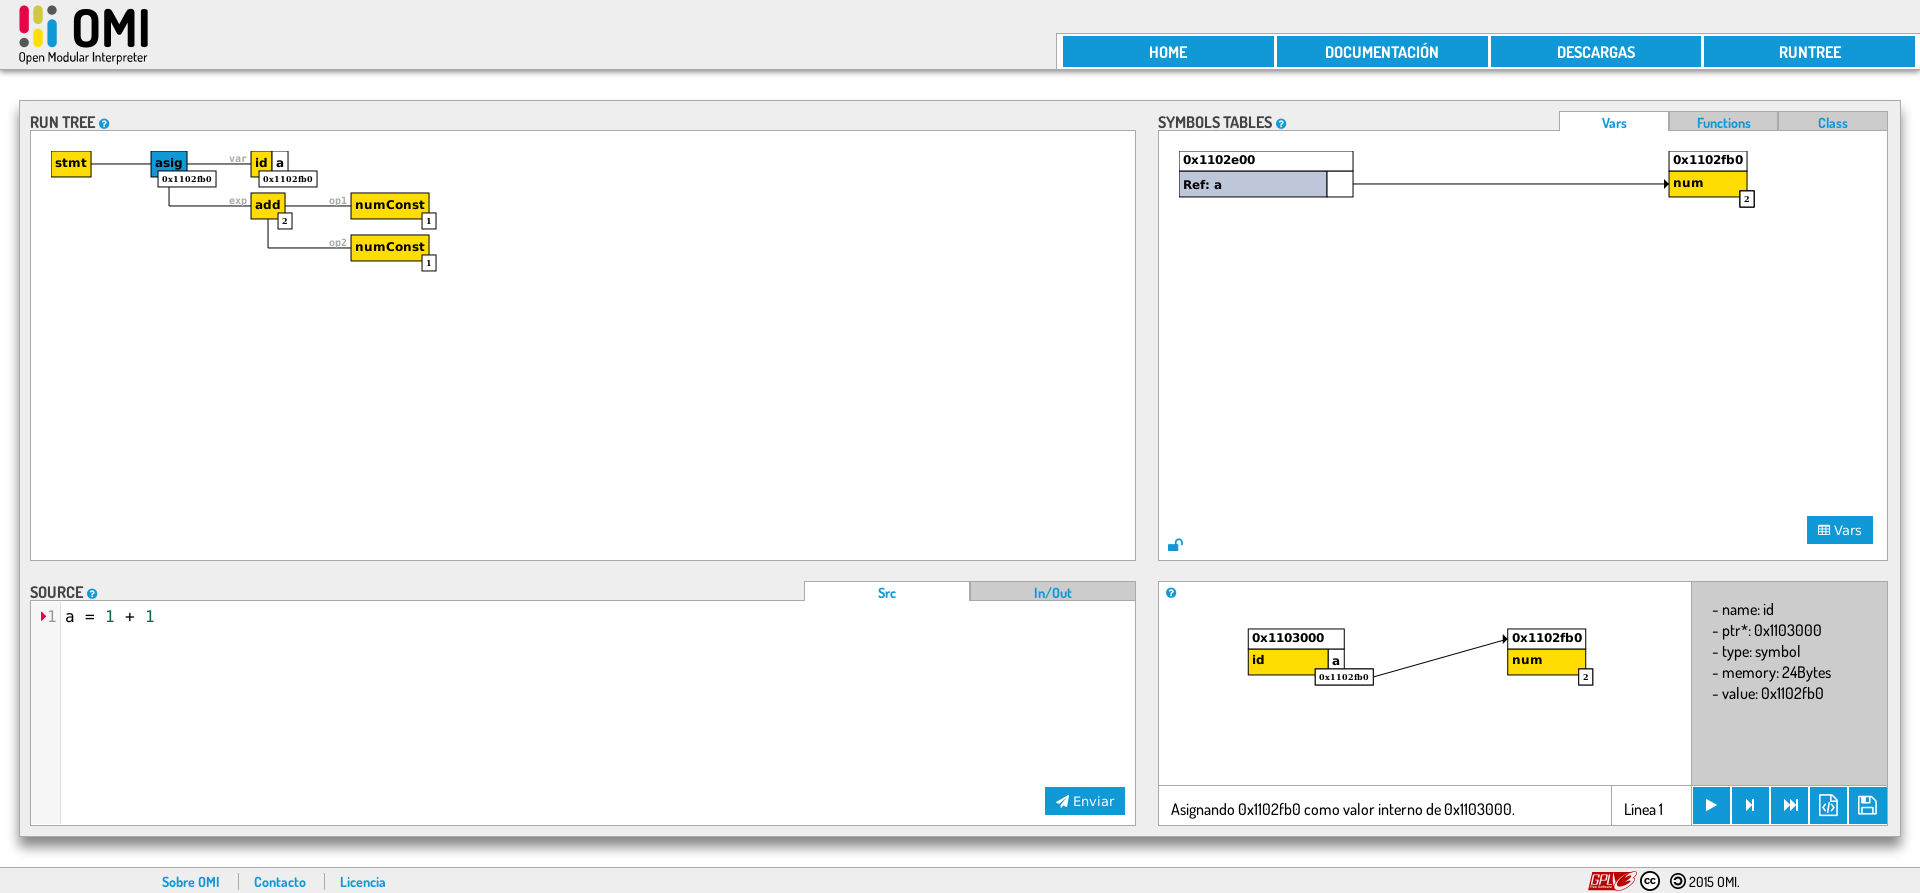
\includegraphics[scale=0.2]{runtree.png} \\
\end{center}

La primera parte de la retícula, superior izquierda, muestra el árbol sintáctico correspondiente al código enviado. En este árbol se marcarán los nodos a medida 
que se van ejecutando y resolviendo semánticamente. Además mostrará información directa de cada nodo tal como el nombre, el valor o el tipo.

En la segunda parte, superior derecha, muestra las tablas de símbolos de variables, funciones y clases. Esta sección permite navegar por las tablas de símbolos 
y los elementos que serán referenciados desde las mismas.

En la tercera parte, inferior izquierda, se muestra el código fuente y la interfaz de entrada/salida del programa.

En la última sección, inferior derecha, se muestra una consola informativa, en la que aparece una descripción del nodo actualmente en ejecución o 
los nodos seleccionados por el usuario. También se colocan en esta sección las opciones de control para avanzar un paso, una sentencia, la reproducción automática, abrir un fichero local o guardar el 
código en un fichero local. 

\subsection{Sitio web}
Según el análisis de la interfaz de usuario llevado a cabo se procede a detallar gráficamente cada página descrita.

\subsubsection{Home}
\begin{center}
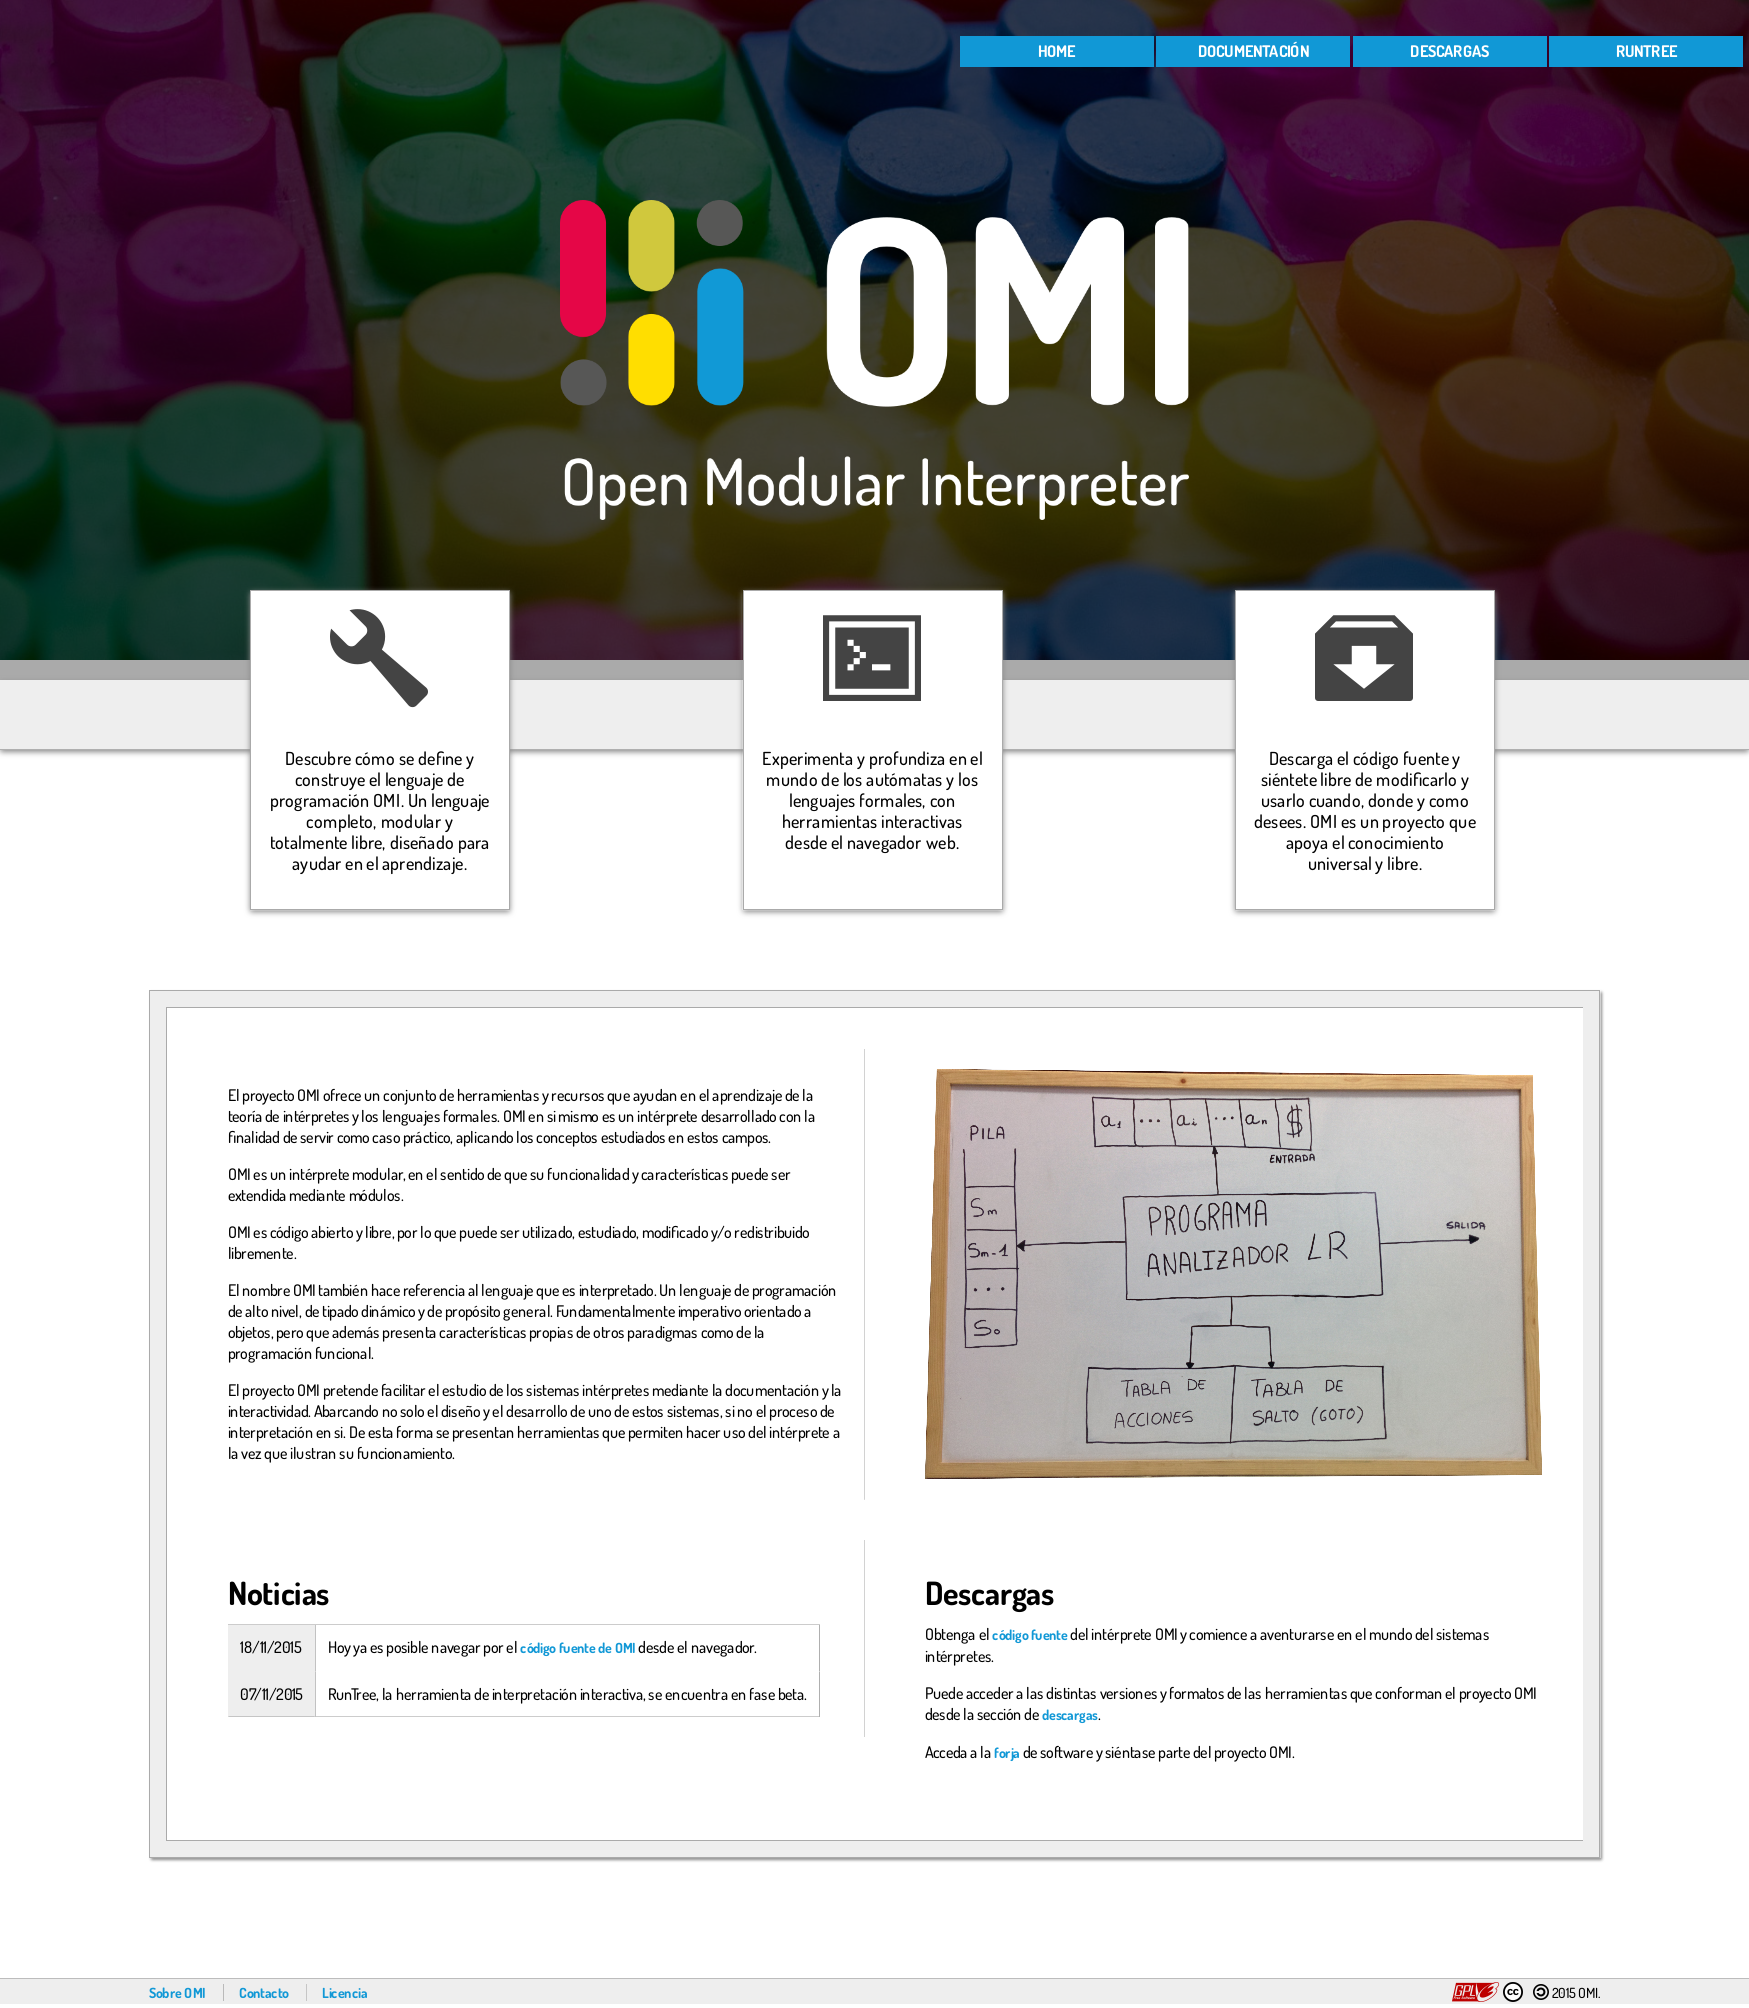
\includegraphics[scale=0.2]{home.png} \\
\end{center}

\subsubsection{Sobre OMI}
\begin{center}
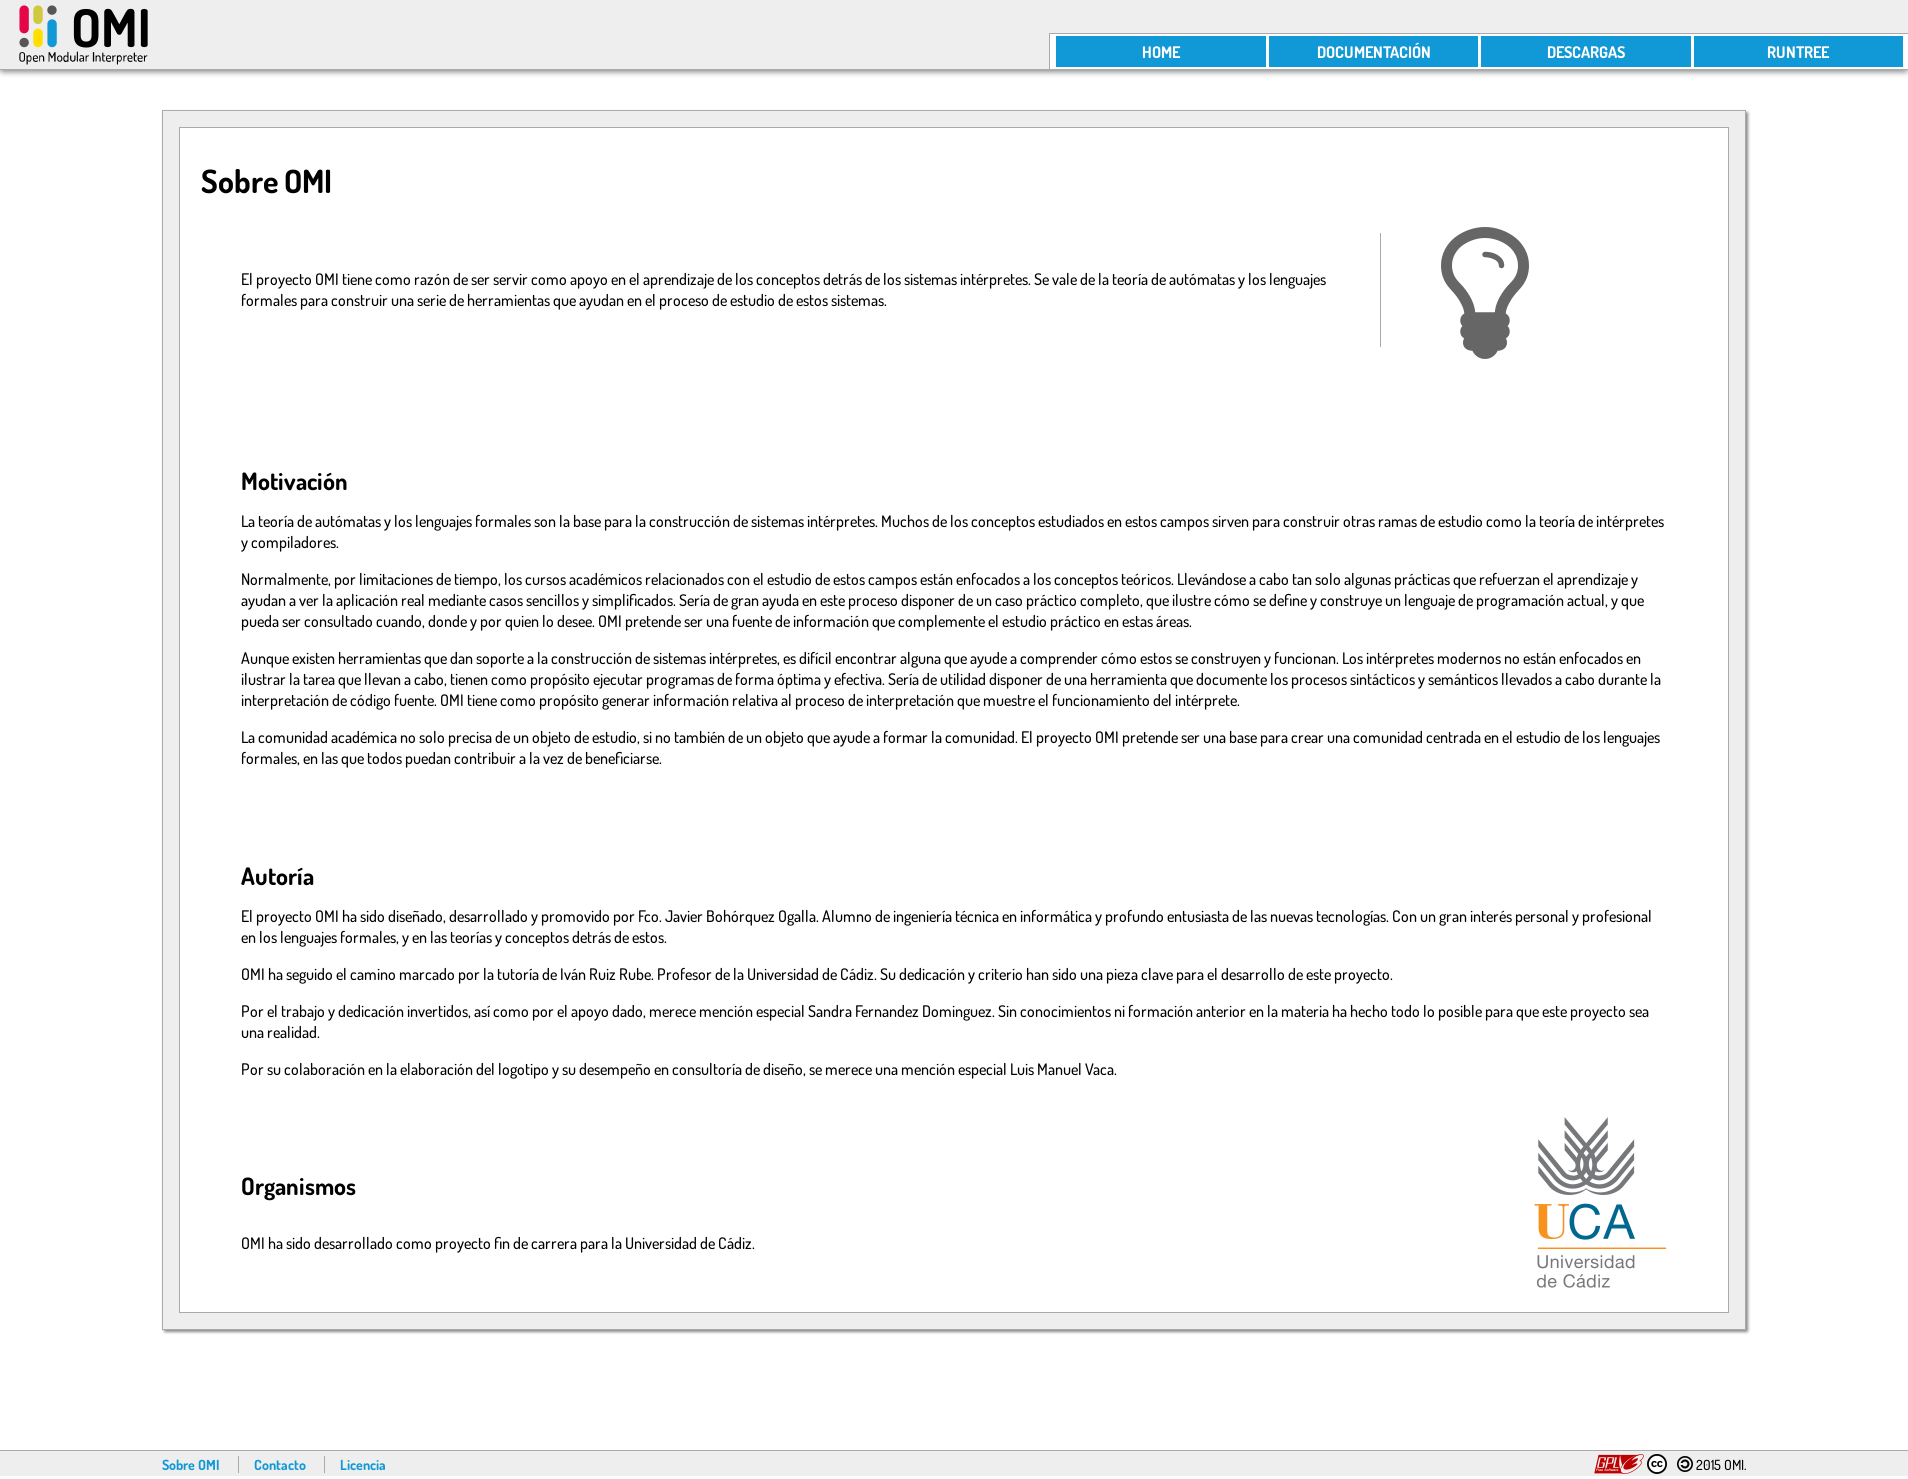
\includegraphics[scale=0.2]{about.png} \\
\end{center}

\subsubsection{Contacto}
\begin{center}
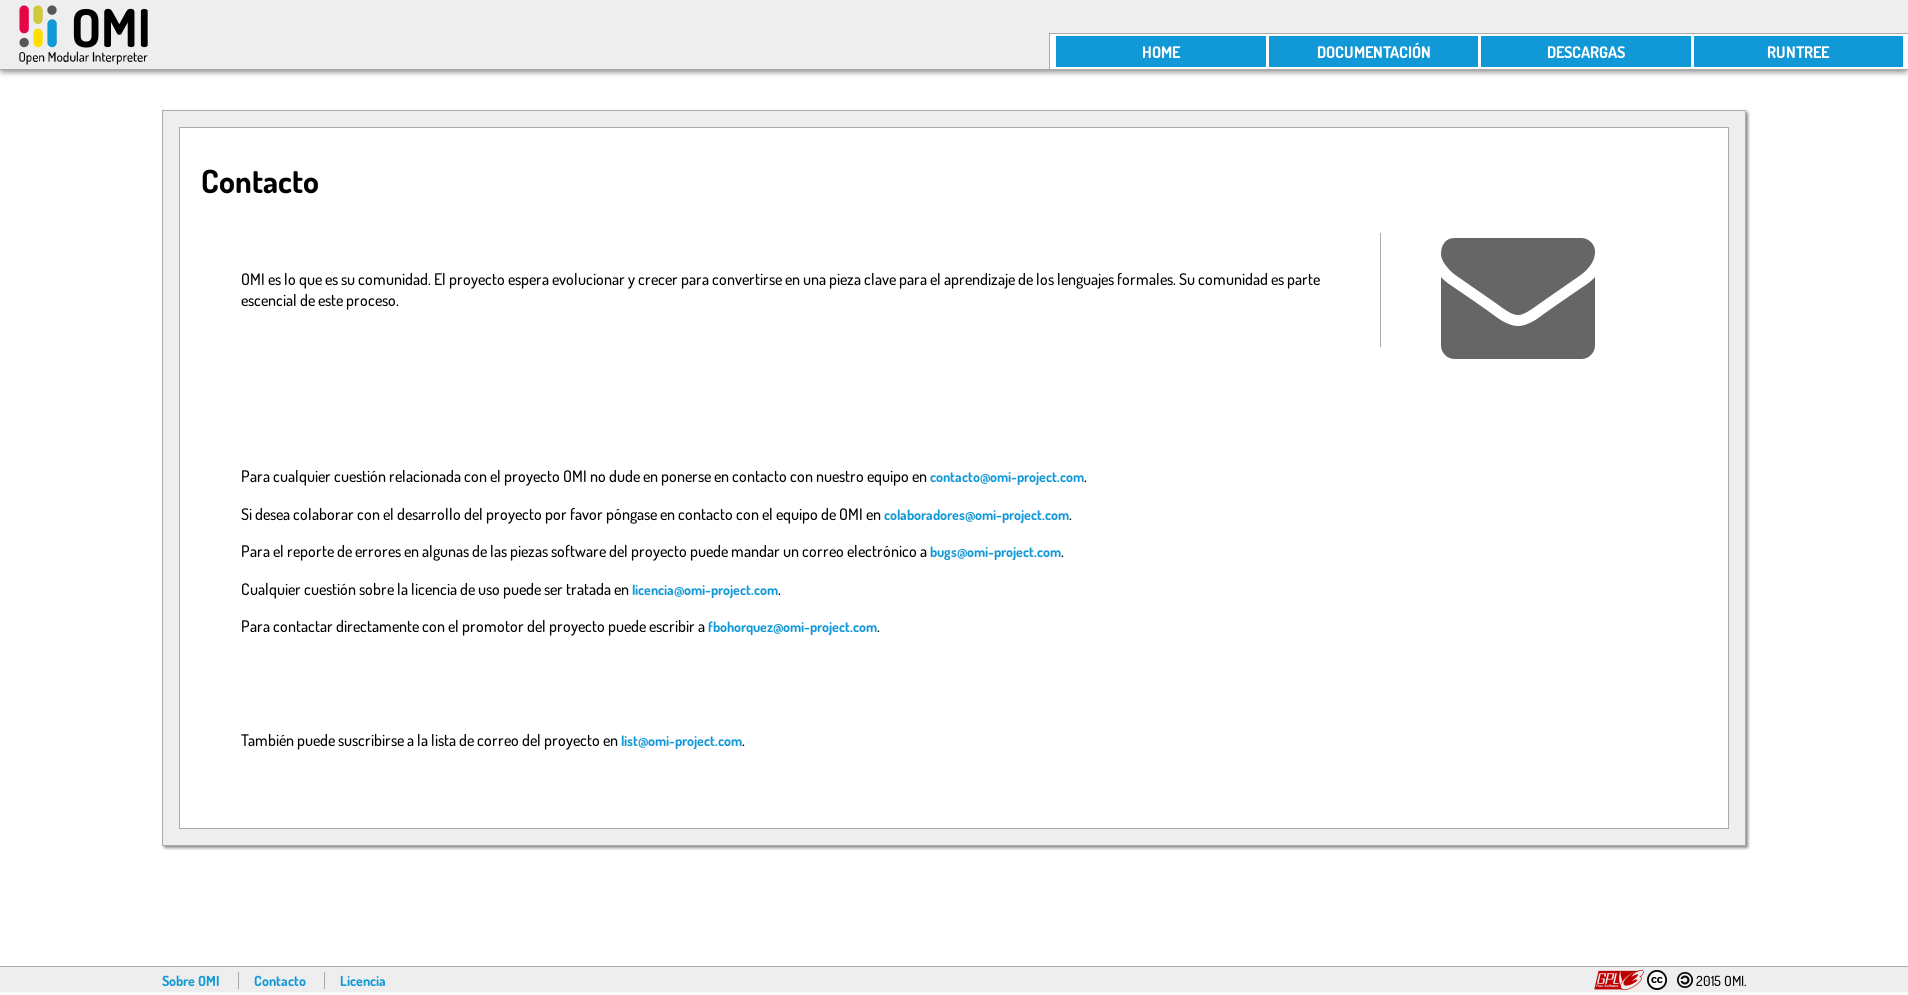
\includegraphics[scale=0.2]{contact.png} \\
\end{center}

\subsubsection{Índice de la documentación}
\begin{center}
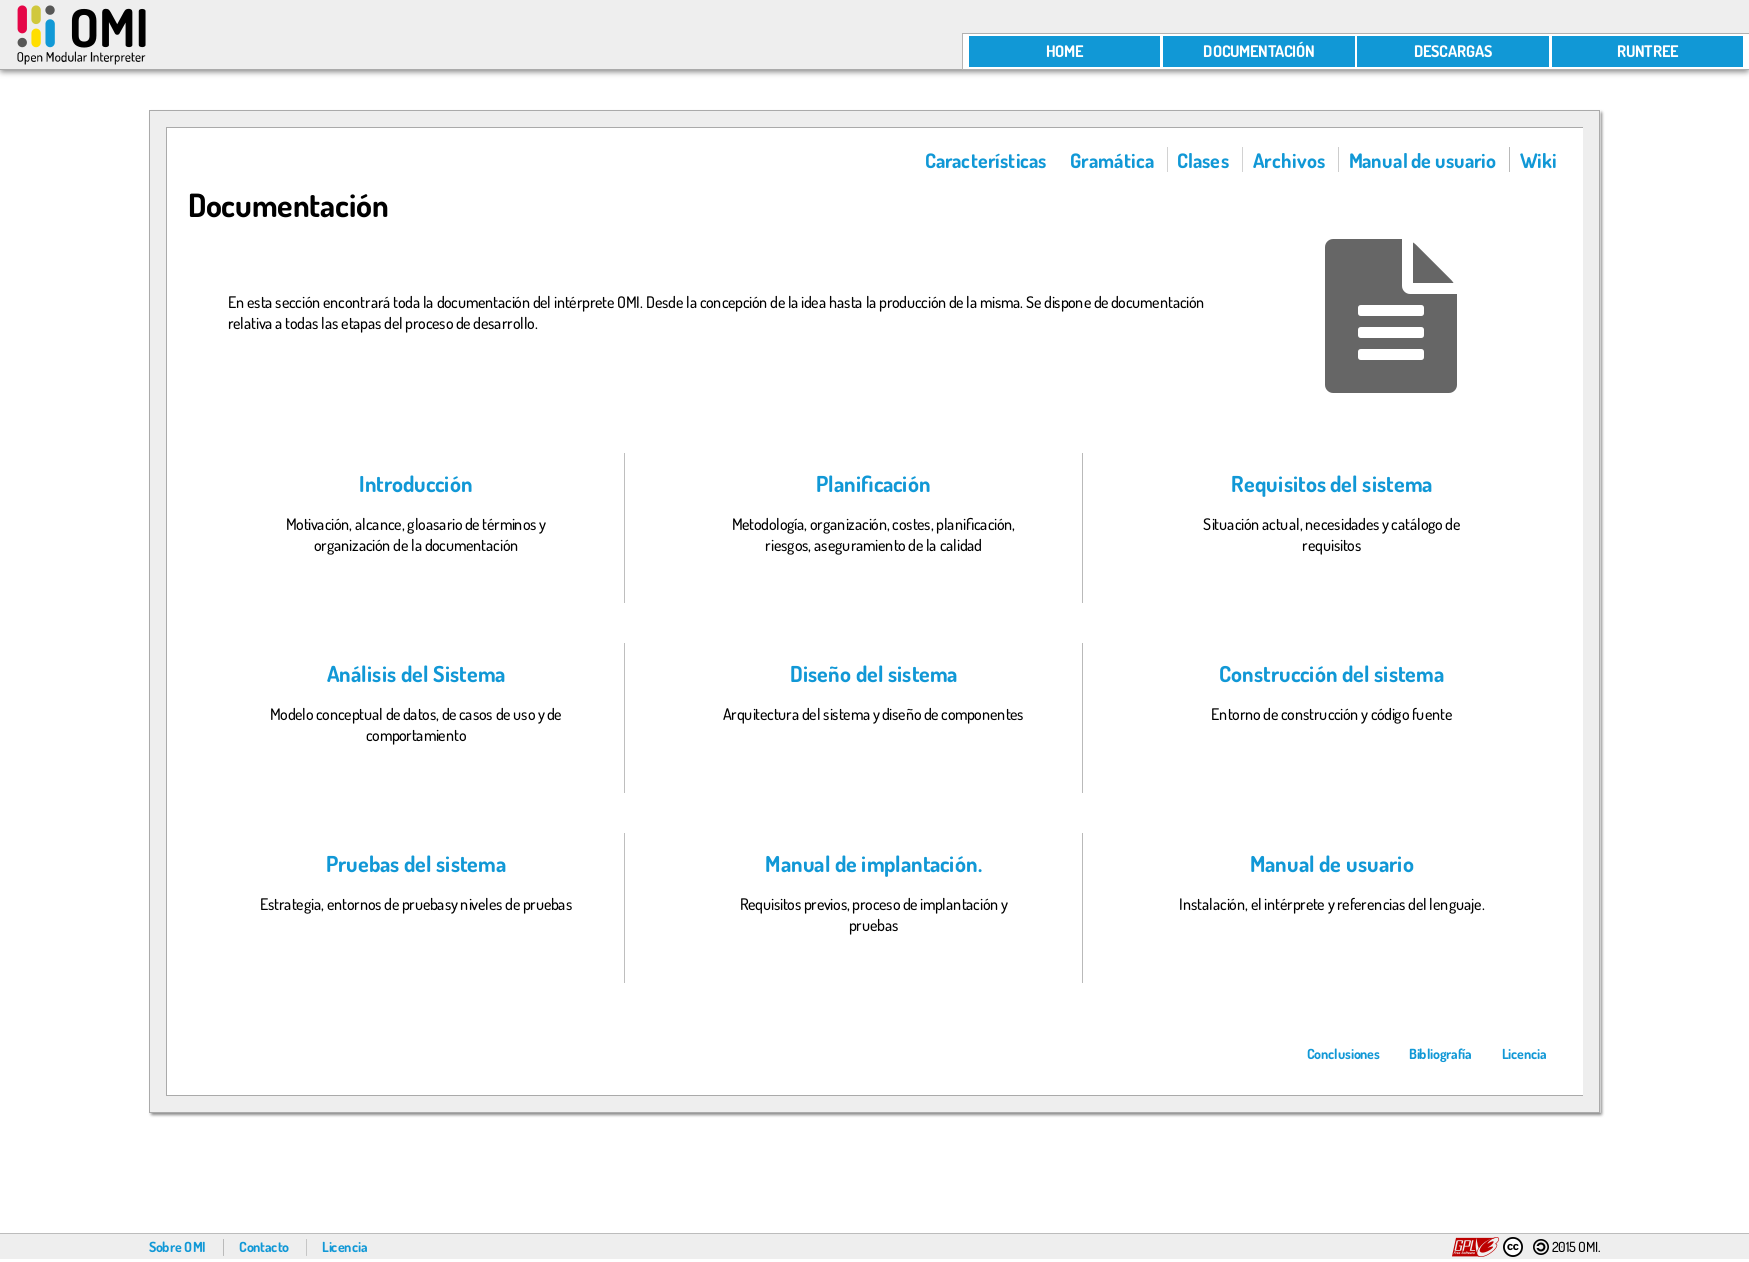
\includegraphics[scale=0.2]{doc-index.png} \\
\end{center}

\subsubsection{Documento}
\begin{center}
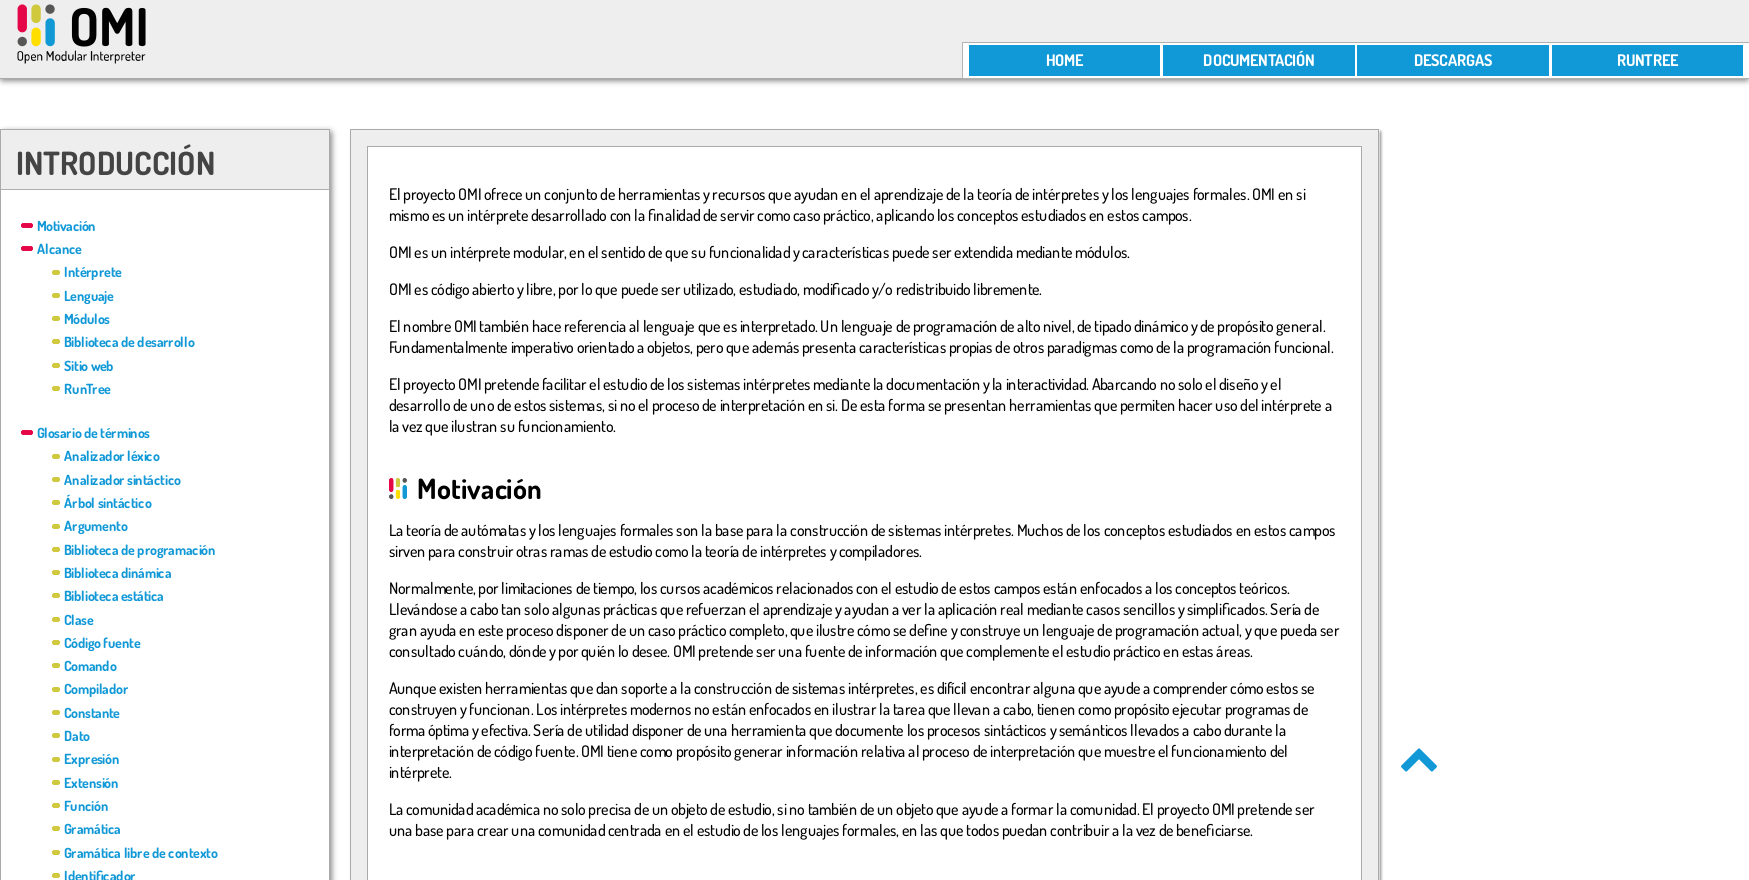
\includegraphics[scale=0.2]{doc-content-x.png} \\
\end{center}

\subsubsection{Navegador de gramática}
\begin{center}
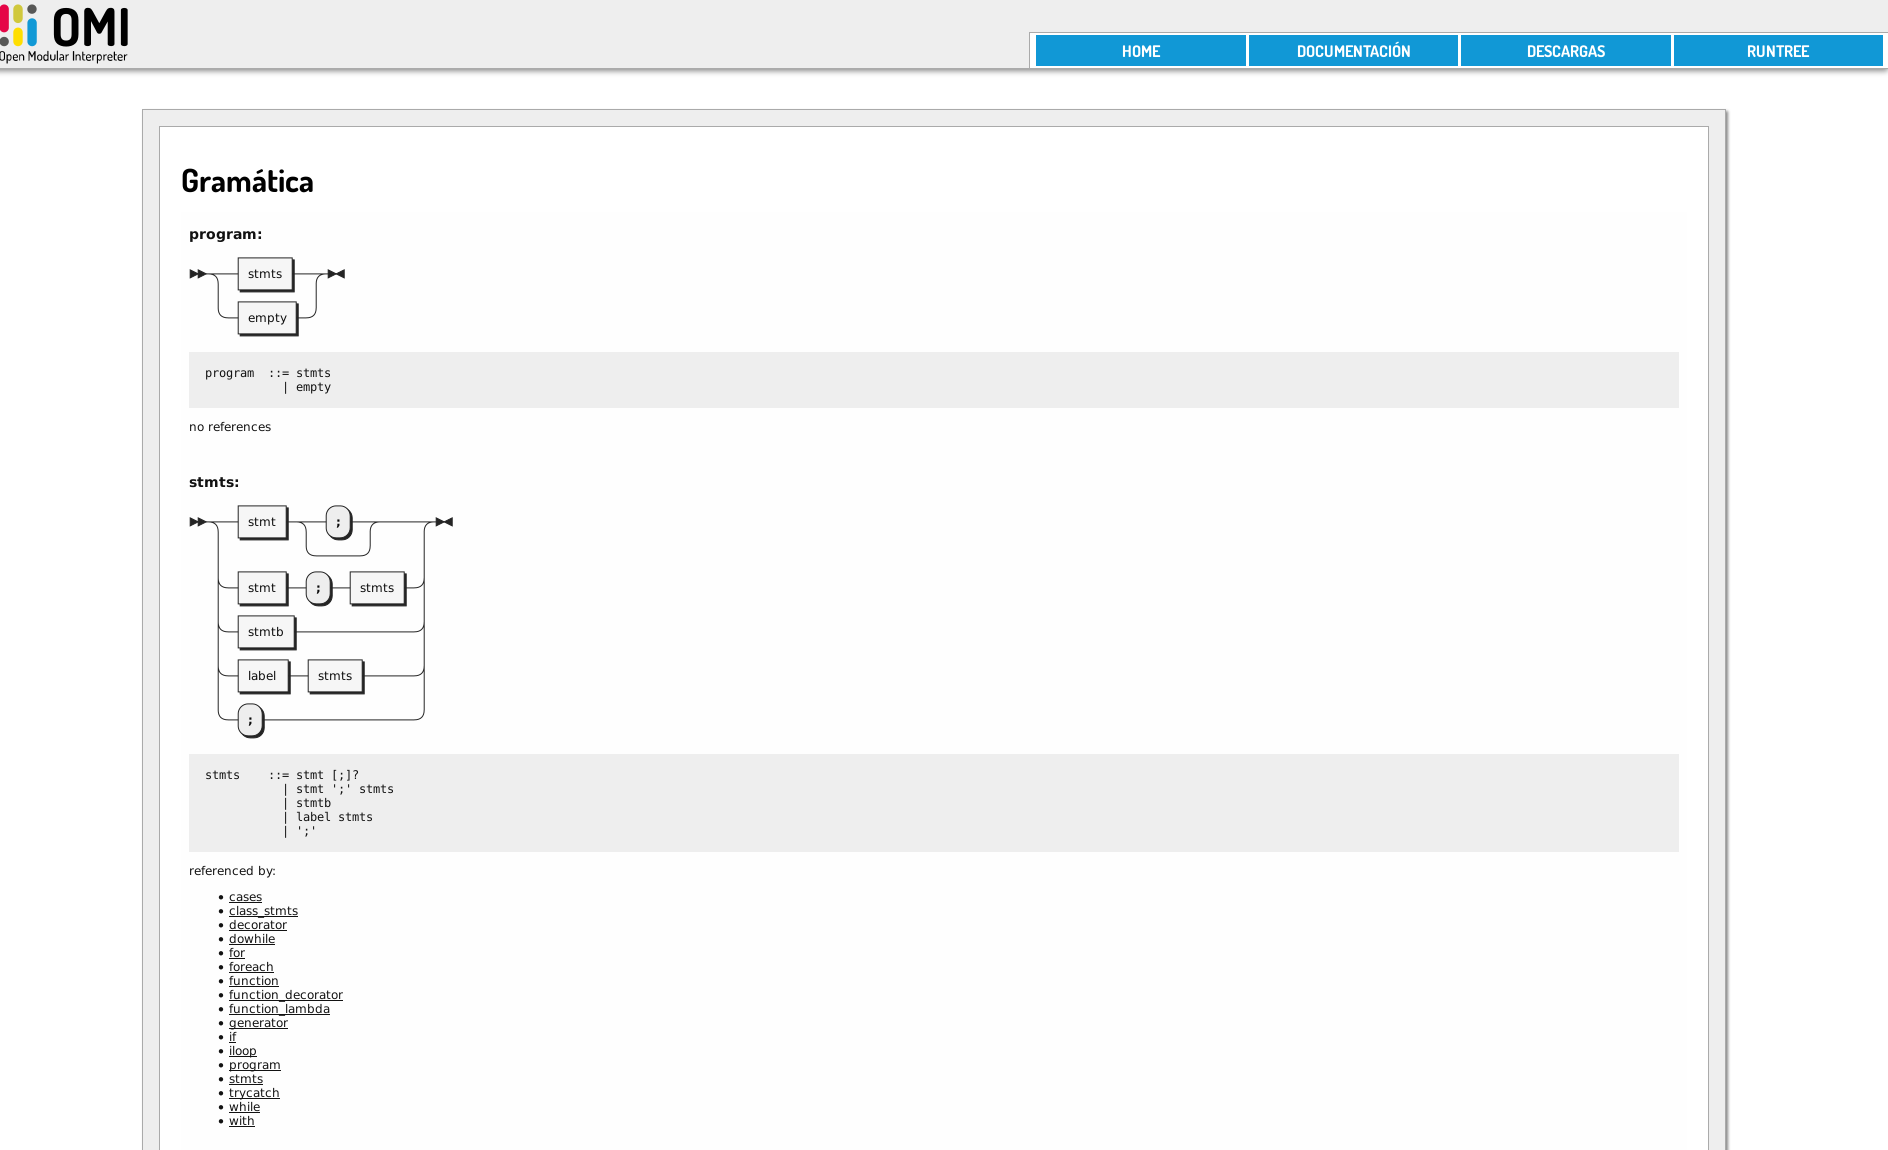
\includegraphics[scale=0.2]{gramatic-x.png} \\
\end{center}

\subsubsection{Navegador de clases}
\begin{center}
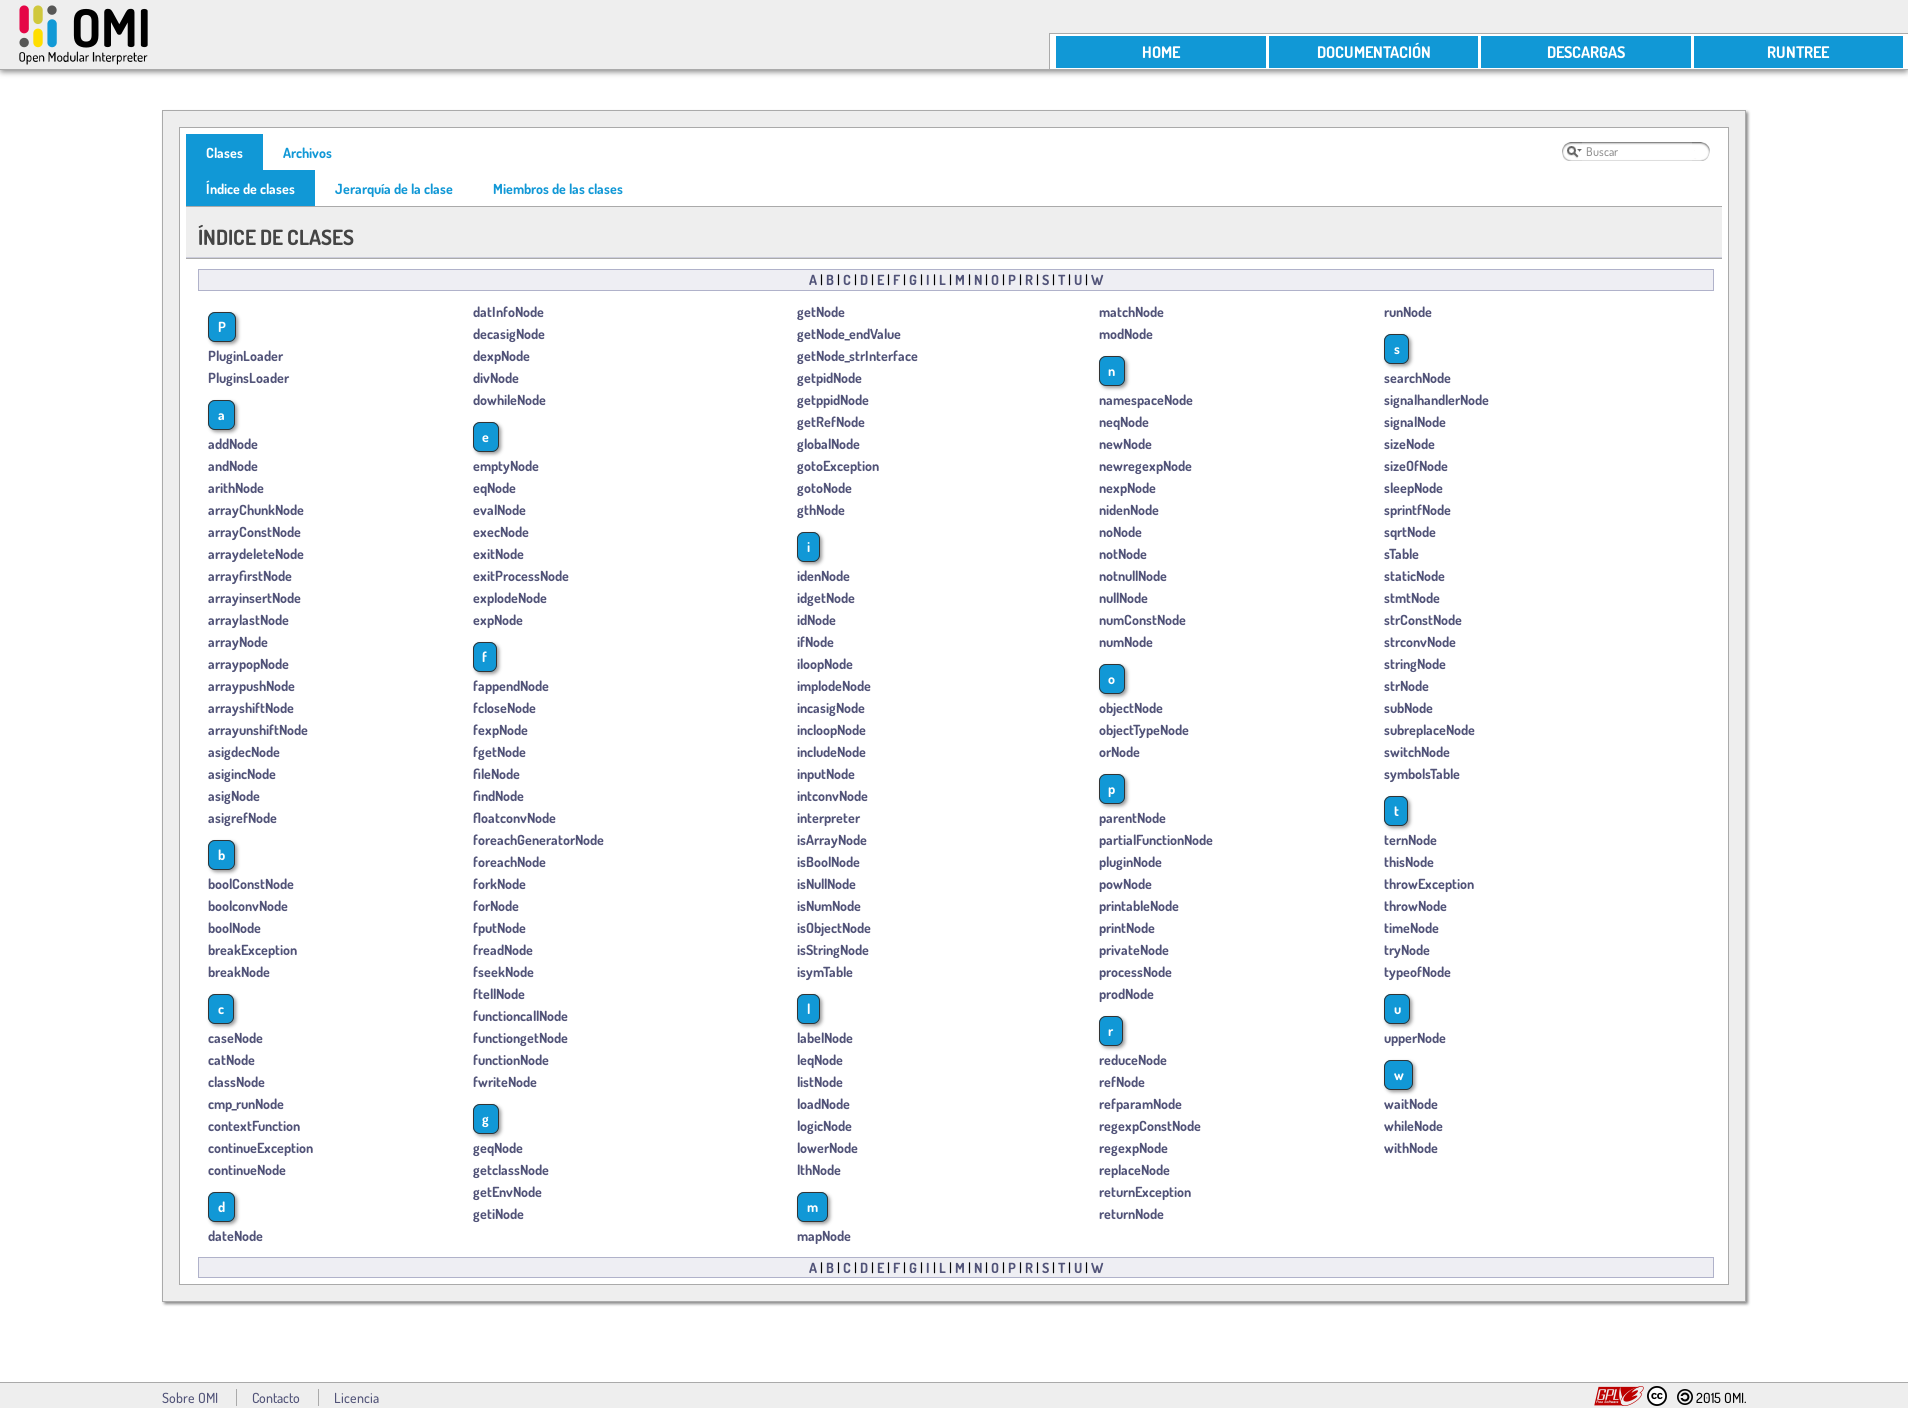
\includegraphics[scale=0.2]{class.png} \\
\end{center}

\subsubsection{Navegador de ficheros}
\begin{center}
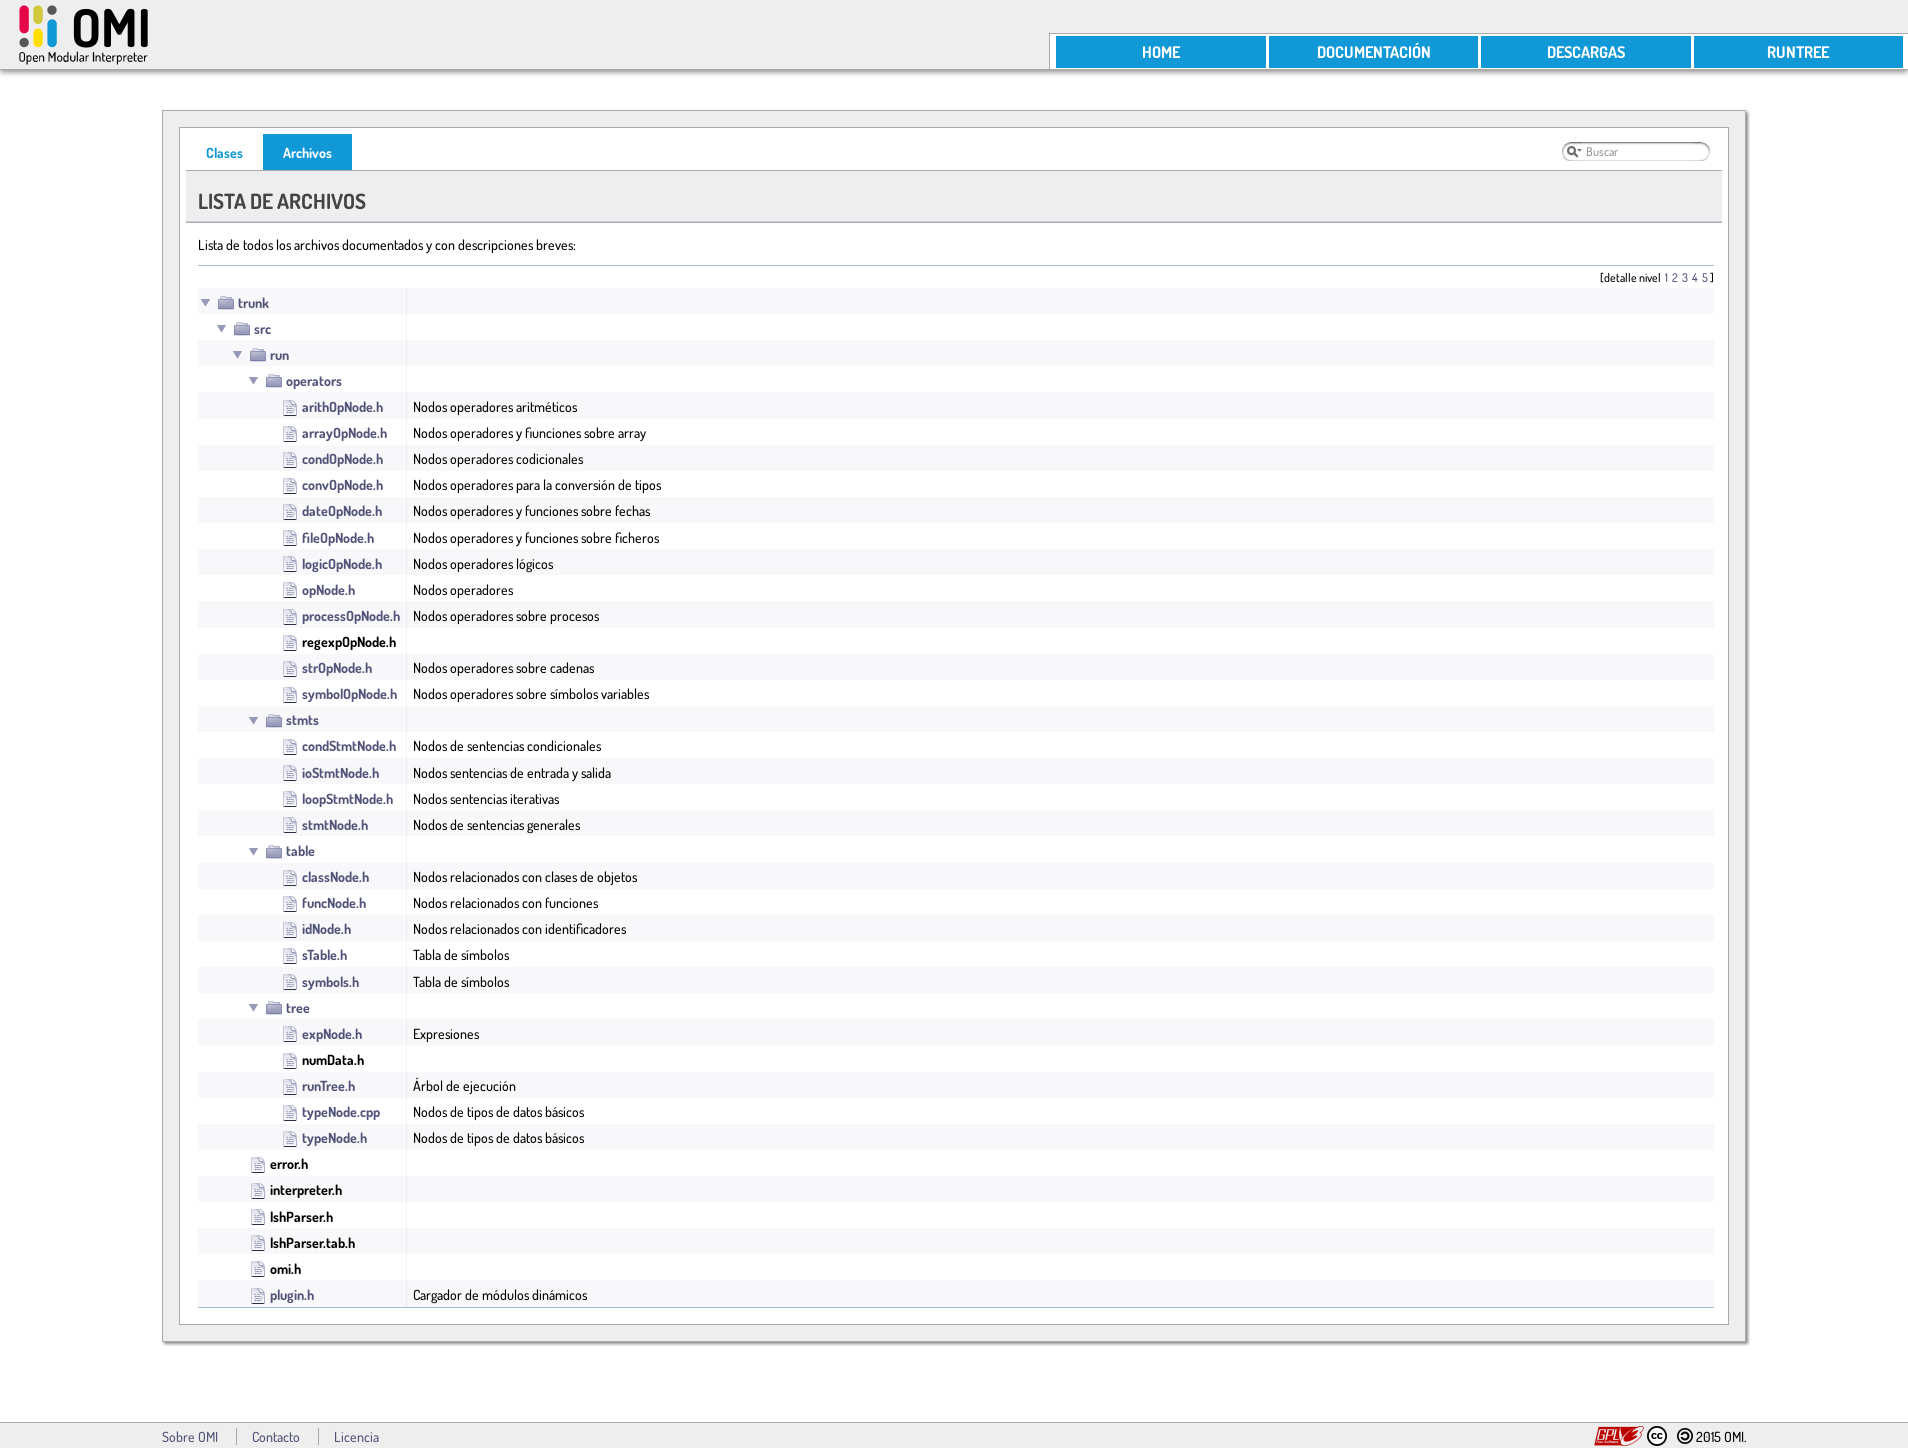
\includegraphics[scale=0.2]{files.png} \\
\end{center}

\subsubsection{Descargas}
\begin{center}
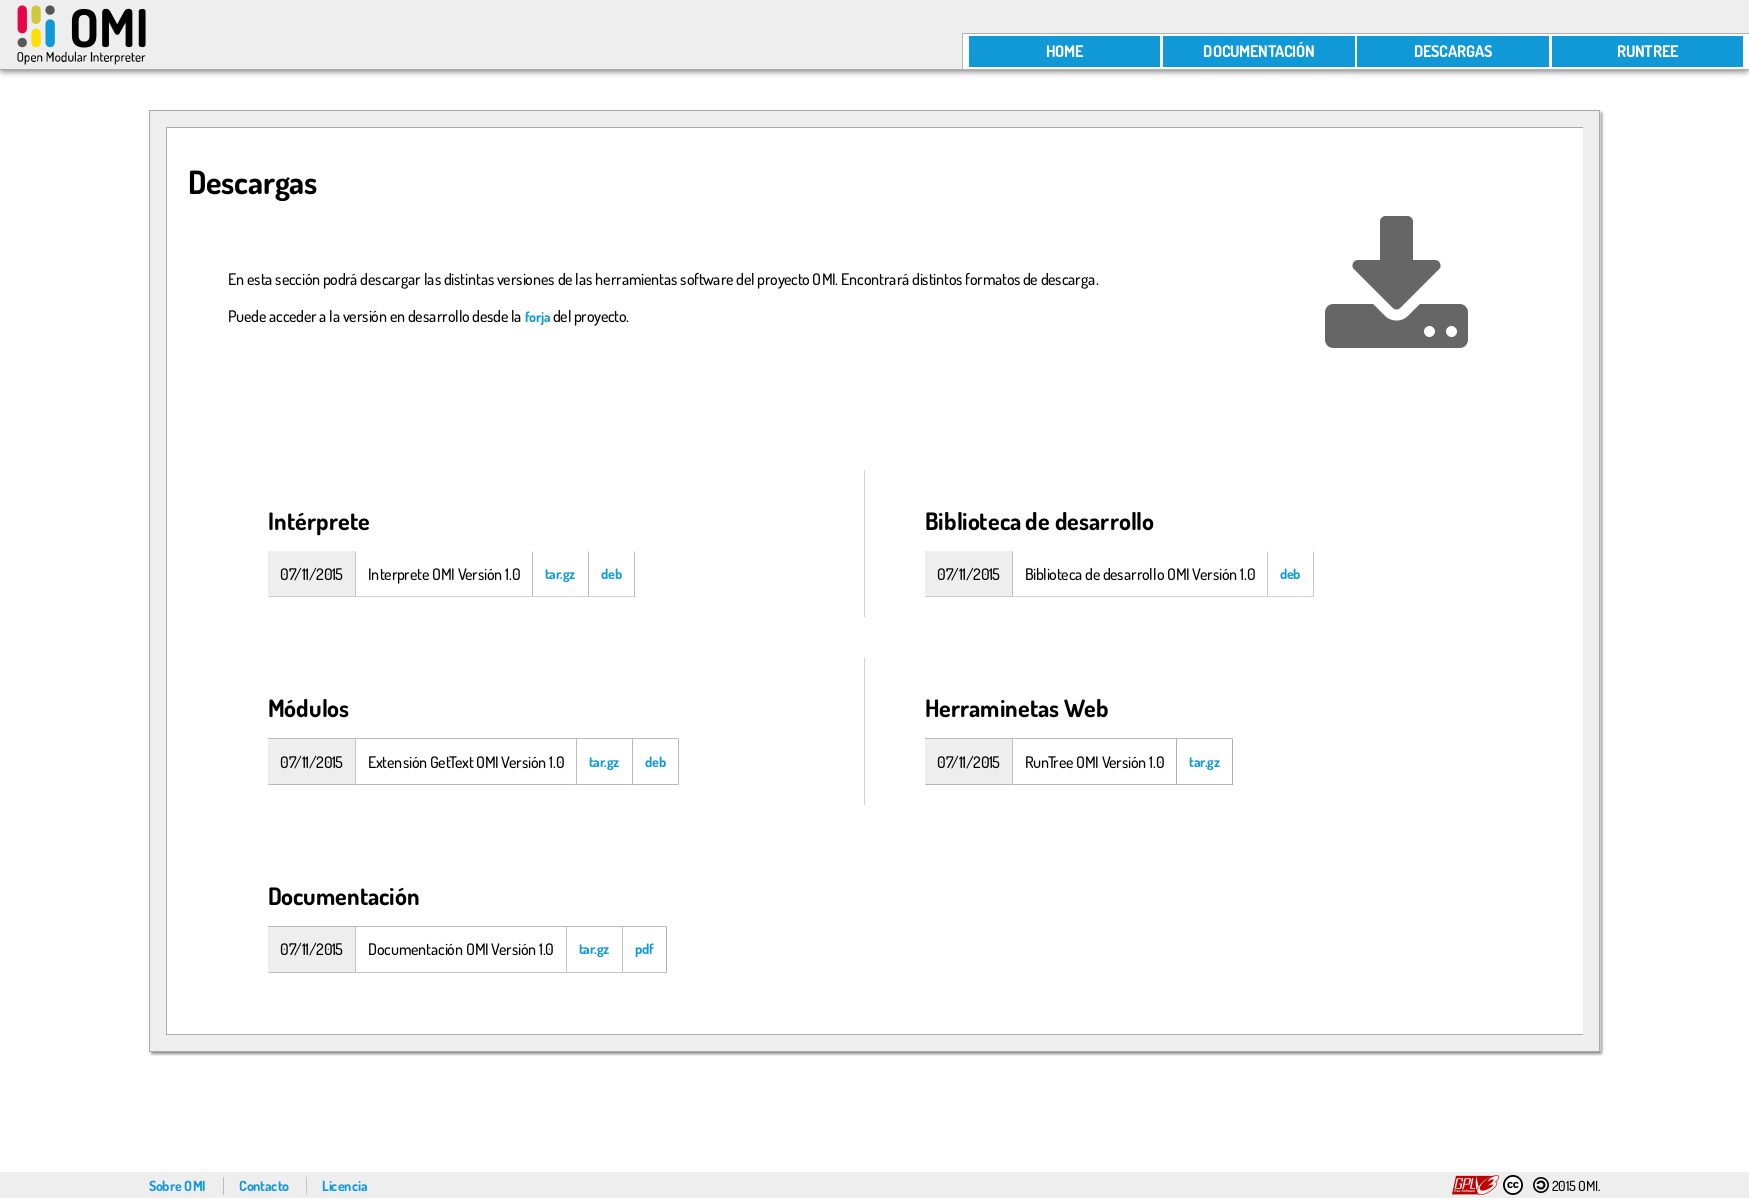
\includegraphics[scale=0.2]{download.png} \\
\end{center}

\end{document}
%%%%%%%%%%%%%%%%%%%%%%%%%%%%%%%%%%%%%%%%%%%%%%%%%%%%%%%%%%%%%%%%%%%%%%%%
%Fco. Javier Bohórquez Ogalla
